\section{Polynomials}
\label{ch:polinomi}

The concept of a ``polynomial'' is an abstraction that is not easily formalized.
In Chapter~\ref{ch:edo}, it will be very useful to apply a polynomial to a
differential operator, and thus we now aim to make very clear what we mean by a
polynomial. In particular, we will distinguish three concepts that are often
conflated: \emph{polynomial expression}, \emph{polynomial}, and \emph{polynomial
function}.

If $A$ is an abelian ring with unity (definition~\ref{def:anello}, for example
$A=\ZZ$, $A=\QQ$, $A=\RR$, or $A=\CC$), we can consider all expressions
(formally: evaluation trees) that can be constructed using the operations of
addition and multiplication involving coefficients taken from $A$ and a variable
we can call $x$ (and more generally, it is possible to consider polynomials in
several variables). These expressions will be called \emph{polynomial
expressions}%
\mymargin{polynomial expressions}%
\index{expressions!polynomial} over $A$ (or with coefficients in $A$) in the variable $x$. An example of a polynomial expression is shown in Figure~\ref{fig:49389}.
\begin{figure}
\begin{center}
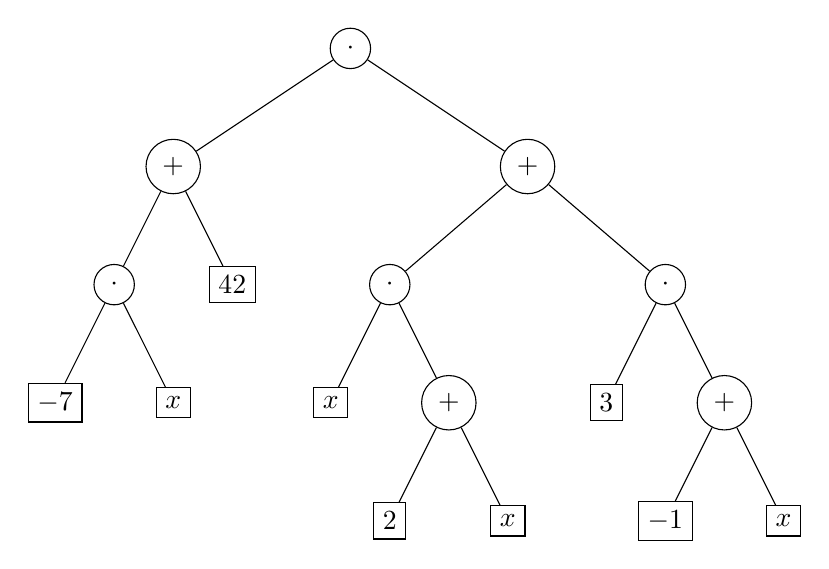
\begin{tikzpicture}
\node [circle,draw] {$\cdot$}
  child {
    node [circle,draw,xshift=-15mm] {$+$}
    child {
      node [circle,draw] {$\cdot$}
      child {node [draw]{$-7$}}
      child {node [draw]{$x$}}
    }
    child {node [draw] {$42$}}
  }
  child {
    node [circle,draw,xshift=15mm] (M) {$+$}
    child {
      node [circle,draw,xshift=-10mm]{$\cdot$}
      child {node [draw]{$x$}}
      child {
        node [circle,draw]{$+$}
        child {node [draw] {$2$}}
        child {node [draw] {$x$}}
        }
      }
    child {
      node [circle,draw,xshift=10mm]{$\cdot$}
      child {node [draw] {$3$}}
      child {
        node [circle,draw] {$+$}
        child {node [draw] {$-1$}}
        child {node [draw] {$x$}}
        }
    }
  };
\end{tikzpicture}
\end{center}
\caption{The polynomial $P = \enclose{(-7)\cdot x + 42}\cdot(x\cdot (2+x) + 3\cdot(-1+x))$ represented as an evaluation tree.}
\label{fig:49389}%
\end{figure}
Polynomial expressions can be added and multiplied together to obtain new
expressions. As a convenient notation, integer powers are used to denote
repeated multiplication $n$ times: $x^n = x\cdots x$.

We will say that two expressions are \emph{equivalent} if it is possible to
transform one into the other using the properties valid in abelian rings:
associative and commutative properties for addition and multiplication,
distributive property, identity elements $1\cdot x = x$, $0 + x = x$. Moreover,
if a branch of the expression does not contain the variable $x$, it is possible
to evaluate (in the ring $A$) the operations and replace the entire branch with
the result of such operations (and vice versa).

In particular, if we have any expression, we can expand all products using the
distributive property and then reassociate the terms with the same powers of
$x$, for example:
\begin{align*}
P &= \enclose{(-7)\cdot x+42}\cdot(x\cdot (2 + x)
+ 3\cdot(-1+x))\\
&= \enclose{(-7)\cdot x + 42}\cdot (2x+x^2-3+3x) \\
% (42-7x)  *  (-3 + 5x + x^2)
&= 126 + 231 x + 7 x^2 - 7 x^3
\end{align*}
In general, we will obtain a polynomial expression that we will say is in
\emph{canonical form}:
\[
  P = a_0 + a_1 x + a_2 x^2 + \dots + a_n x^n
       = \sum_{k=0}^n a_k x^k.
\]
Thus, every polynomial expression is equivalent to a polynomial expression in
canonical form.

If two polynomial expressions are equivalent, we will say that they represent
the same \emph{polynomial}%
\mymargin{polynomial}%
\index{polynomial}.
If $A$ is a ring, we will denote by 
$A[x]$ \index{$\KK[x]$}\index{$A[x]$}%
the set of all polynomials with coefficients in $A$ and variable $x$. 
Formally, $A[x]$ is the quotient of the set 
of all polynomial expressions with respect to the equivalence relation
we have just defined. 
We can add and multiply polynomials, and these operations 
make $A[x]$ itself a ring.

More explicitly, if $P$ and $Q$ are polynomials in canonical form
\[
  P = \sum_{k=0}^n a_k x^k, \qquad Q = \sum_{k=0}^m b_k x^k
\]
we will have:
\[
  P + Q = \sum_{k=0}^{N} (a_k+b_k) \cdot x^k
\]
where $N$ is the largest of $n$ and $m$, and it is understood that $a_k=0$ for
$k>n$ and
$b_k=0$ for $k>m$.
If $t\in A$, we will have:
\[
  t P = \sum_{k=0}^n (ta_k)\cdot x^k.
\]
Regarding the product, we will have:
\begin{align*}
  P\cdot Q
  &= \enclose{\sum_{k=0}^n a_k x^k}\cdot \enclose{\sum_{j=0}^n b_j x^j}
  = \enclose{\sum_{k=0}^n a_k \enclose{\sum_{j=0}^m b_j x^j} x^k} \\
  &= \enclose{\sum_{k=0}^n \sum_{j=0}^m a_k b_j x^{j+k}}
  = \sum_{s=0}^{m+n} \enclose{\sum_{j=0}^s a_j b_{s-j}} x^s.
\end{align*}

The formulas for the sum and product of polynomials in canonical form 
can be applied to each of the ring properties to demonstrate
that equivalent polynomials have the same canonical form and that therefore 
two polynomial expressions are equivalent if and only if the coefficients 
of their canonical form coincide.
In practice, polynomials with coefficients in $A$ are 
represented by the coefficients of their canonical forms, which 
are nothing but finite sequences:
\begin{align*}
  A[x] 
  &= \{\sum_{k=0}^n a_k x^k\colon a_k\in A, n\in \NN\}\\
  &\approx A^\NN_c 
    = \ENCLOSE{\vec a \in A^\NN\colon \ENCLOSE{k\in \NN\colon \vec a(k)\neq 0}
  \text{ is finite}}.
\end{align*}

If the polynomial $P$ is written in canonical form
\[
  P = \sum_{k=0}^n a_k x^k
\]
if $n>0$, we can assume that the coefficient $a_n$ is different from $0$ 
because otherwise, we could remove the corresponding term and reduce 
to a sum of $n-1$ terms. 
In such a case, we will say that the polynomial $P$ has \emph{degree}%
\mymargin{degree}%
\index{degree} $n$.
\index{polynomial!degree}%
\index{degree!polynomial}% 
If $n=0$, we will also say that the polynomial is constant.
If $n=0$ and $a_n=0$, we will say that $P$ is the \emph{zero} polynomial.
Non-zero constant polynomials have a degree equal to $0$, while the zero
polynomial,
by convention, is said to have a degree of $-\infty$ (this definition makes
sense if one thinks
of the degree of a polynomial as the smallest number for which all coefficients
of
index greater than it are zero).

So far, we have defined the polynomial as an equivalence class of 
polynomial expressions. 
If we take an expression $P$ and replace the variable $x$ 
with an element $a$ of the ring $A$ (or of any ring that extends 
$A$), then we can evaluate all operations (sums and products) and 
obtain a result in the chosen ring: the result 
obtained is denoted by $P(a)$ (the same notation used for functions).
If $P$ is a polynomial in the variable $x$, the function $x\mapsto P(x)$ 
can be called a \emph{polynomial function}%
\mymargin{polynomial function}%
\index{function!polynomial} and is usually denoted 
with the same name $P$ given to the polynomial. The context will tell us 
whether $P$ refers to the polynomial (the expression) or the function.

As already mentioned, it is useful to keep the concept of a polynomial separate
from that of a
polynomial function because the same polynomial can be evaluated over different 
rings (for example, in the course of geometry, one might substitute
the variable $x$ of a polynomial with a matrix, 
and in the last chapter of these notes, 
we will substitute $x$ with a differential operator).

We will continue with the treatment of polynomials 
in Chapter~\ref{ch:ancora_polinomi}, 
when we can address the fundamental theorem of algebra.

\subsection{Notable Products}
\label{sec:prodotti_notevoli}

It will often happen to encounter certain particular polynomials, which are 
sometimes called \emph{notable products}%
\mymargin{notable products}%
\index{product!notable}. 
Of fundamental importance are those of degree 2:
\[
  (x+1)\cdot(x-1) = x^2-1, \qquad (x+1)^2 = x^2+2x + 1.
\]
But also those of degree $n$:
\[
(x-1)\cdot(1+x+x^2+\dots + x^{n-1}) = x^n - 1
\]
which is formally written (and proven) as follows:
\begin{equation}\label{eq:933456}
  (x-1)\cdot \sum_{k=0}^{n-1} x^k
  = \sum_{k=0}^{n-1} x^{k+1} - \sum_{k=0}^n x^k = x^n - 1.
\end{equation}
We have thus found the formula, valid for $x\neq 1$
(possibly also $x\in \CC$):
\[
  \sum_{k=0}^{n-1} x^k = \frac{x^n-1}{x-1}.
\]
See also exercise~\ref{ex:somma_geometrica}.
A progression of the type $1,x,x^2,x^3,\dots$ has the property 
that the ratio of two consecutive terms is constant (equal to $x$).
It is called a \emph{geometric progression}.
\index{geometric progression}%
\mymargin{geometric progression}%
What we have 
found is thus the formula for calculating the sum of the first $n$ terms of 
such a progression.
Note that the \emph{geometric} progression is analogous to an \emph{arithmetic}
progression if we replace multiplication with addition.
In fact, in arithmetic progressions, it is the difference between two
consecutive terms
that is constant 
(the sum of an arithmetic progression can be calculated as 
in exercise~\ref{ex:somma_lineare}).

By substituting $-x$ for $x$ in~\eqref{eq:933456} 
and changing the sign, we obtain:
\[
  (x+1)\cdot \sum_{k=0}^{n-1} (-1)^k x^k
  = 1 + (-1)^n x^n
\]
that is,
\[
(x+1)\cdot (1-x+x^2- \dots + (-1)^{n-1} x^{n-1}) = 1 + (-1)^n x^n.
\]

\subsection{Relation between Arithmetic Mean and Geometric Mean}

The notable products listed in the previous section are valid 
in any ring, in particular, it can be $x\in \RR$ but also $x \in \CC$.

However, if we remain in the case $x\in \RR$, we know that $x^2\ge 0$
and we can obtain useful inequalities.
Starting from
\[
0 \le (x-y)^2 = x^2 + y^2 - 2xy
\]
we obtain Young's inequality:
\mymargin{Young's inequality}%
\index{inequality!Young's}%
\[
xy \le \frac{x^2+y^2}{2}
\]
and consequently:
\[
 (x+y)^2 = x^2 + y^2 + 2xy \ge 2xy + 2xy = 4 xy
\]
which, if $x\ge 0$ and $y\ge 0$, can be written as:
\mymargin{arithmetic/geometric mean}%
\index{mean!arithmetic}%
\index{mean!geometric}%
\index{inequality!arithmetic/geometric mean}%
\index{AM}%
\index{GM}%
\[
   \frac{x+y}{2} \ge \sqrt{xy}.
\]
The expression $\frac{x+y}{2}$ is the \emph{arithmetic mean}
(for English speakers, the acronym AM, \emph{arithmetic mean})
of the numbers $x$ and $y$
while $\sqrt{xy}$ is the \emph{geometric mean}
(for English speakers, the acronym GM, \emph{geometric mean}).

Note that the formula for the geometric mean is obtained from the formula 
for the arithmetic mean by replacing the addition operation with 
the multiplication operation.
In fact, the two means correspond through the logarithm function,
and the inequality is a property of the concavity of the logarithm,  
as we will see in exercise~\ref{ex:AMGM}.

\subsection{Binomial Coefficients}
\label{ch:binomiale}

The powers of the binomial $x+1$ are decidedly significant. 
If we write the polynomial $(x+1)^n$ in canonical form:
\[
  (x+1)^n = \sum_{k=0}^n a_k x^k  
\]
we would be interested in calculating the value
of the coefficients $a_k$. 
First of all, we give them a name: these coefficients are called 
\emph{binomial coefficients}%
\mymargin{binomial coefficients}%
\index{binomial coefficients}
\index{binomial!coefficients}%
and are denoted as follows:%
\mynote{%
In the context of combinatorial calculus, 
binomial coefficients 
are also called \emph{combinations}
and denoted with the symbol $C_{n,k} = {n \choose k}$.
The coincidence between combinations and binomial coefficients 
is expressed in theorem~\ref{th:combinatoria}.
}%
\[
    a_k = {n \choose k}.
\]

It is not difficult to convince oneself that if we expand the binomial $(x+y)^n$
the same coefficients are obtained, thus
in general, the following formula holds for the \emph{power of the binomial}%
\mymargin{power of the binomial}%
\index{power!of the binomial}:
\index{binomial!power}% 
\begin{equation*}
  (x+y)^n = \sum_{k=0}^n {n \choose k} x^k y^{n-k}. 
\end{equation*}

To determine the actual value of the binomial coefficients, the following is
usually used.
  
\begin{theorem}[Pascal's Triangle]
\mymark{*}%
\label{th:tartaglia}%
For every $n\in \NN$ and $k \in \NN$ with $1 \le k \le n$, we have
\[
  {n+1 \choose k} =
      {n \choose k-1} + {n \choose k}
\]
while
\[
  {n+1 \choose 0} = 1 = {n+1 \choose n+1}
\]
\end{theorem}
  %
  \begin{proof}
  Indeed, we have 
  \begin{align*}
    \sum_{k=0}^{n+1} {n+1 \choose k} x^k
    &= (1+x)^{n+1} 
    = (1+x)\cdot \sum_{k=0}^n {n \choose k} x^k \\
    &= \sum_{k=0}^n {n\choose k} x^k 
    + \sum_{k=0}^n {n\choose k} x^{k+1}\\
    &= \sum_{k=0}^n {n\choose k} x^k 
    + \sum_{k=1}^{n+1} {n\choose k-1} x^{k}\\
    &= {n\choose 0} x^0 
      + \sum_{k=1}^n \Enclose{{n\choose k} + {n\choose k-1}} x^k
      + {n \choose n} x^{n+1}.
    \end{align*}
  By the uniqueness of the canonical form of polynomials, 
  the corresponding coefficients must be equal, and thus 
  we find
  \[
  {n+1 \choose 0} = {n \choose 0}, \qquad 
  {n+1 \choose k} = {n \choose k} + {n \choose k-1}, \qquad 
  {n+1 \choose n+1} = {n \choose n}.
  \]

  It can be easily verified that  ${0 \choose 0} = 1$, 
  and this concludes the proof.
  \end{proof}
  
  Based on the previous theorem, the binomial coefficients can be
  listed as in Table~\ref{tab:binomiali}:
  each row begins and ends with the number $1$,
  and each intermediate term coincides with the sum of the
  two terms in the previous row above and
  to the left of the considered number.
  
  \begin{table}
  \begin{tabular}{c|ccccccccc}
  $\displaystyle{n \choose k}$& 0 & 1 & 2 & 3 & 4 & 5 & 6 & $k$ &\\ \hline
    0 & 1 &   &   &   &   &   &   & &\\
    1 & 1 & 1 &   &   &   &   &   & &\\
    2 & 1 & 2 & 1 &   &   &   &   & &\\
    3 & 1 & 3 & 3 & 1 &   &   &   & &\\
    4 & 1 & 4 & 6 & 4 & 1 &   &   & &\\
    5 & 1 & 5 & 10& 10& 5 & 1 &   & &\\
    6 & 1 & 6 & 15& 20& 15& 6 & 1 & &\\
  $n$ &$\vdots$&&   &   &   &   &   & $\ddots$ &
  \end{tabular}
  \caption{Pascal's Triangle:
  each number is the sum of the two numbers that are 
  in the previous row above and immediately to the left.}
  \label{tab:binomiali}
  \end{table}
  
  \begin{theorem}[Formula for Binomial Coefficients]
  \mymark{***}%
  If $n\in \NN$ and $k\in \NN$, $k\le n$,
  we have 
  \[
  {n \choose k}  
  = \frac{n!}{k!(n-k)!}.  
  \]
  \end{theorem}
  %
  \begin{proof}
  We prove it by induction on $n$.
  For $n=0$, we know that ${0 \choose 0} = 1$, which 
  is equal to $\frac{0!}{0!0!}$.
  We use theorem~\ref{th:tartaglia}.
  If $k=0$ or $k=n$, we know that ${n \choose k}=1$, which coincides 
  with the stated formula. 
  For the other cases, assuming by induction that the formula is 
  true for a certain $n\in \NN$, we have: 
  \begin{align*}
   {n+1 \choose k} 
   &= {n \choose k} + {n \choose k-1}
   =  \frac{n!}{k!(n-k)!} + \frac{n!}{(k-1)!(n-k+1)!} \\
   &= \frac{n!(n-k+1) + n! k}{k!(n-k+1)!}
   = \frac{n!(n+1)}{k!(n+1-k)!} \\
   &= \frac{(n+1)!}{k!(n+1-k)!}
  \end{align*}
  which is what we needed to prove.
\end{proof}

Note that for every $n\in \NN$:
\[
  {n \choose 1} = {n \choose n-1} = n.
\]
  
\begin{exercise}
  Prove that
  \[
   \sum_{k=0}^n {n \choose k} = 2^n.
  \]
\end{exercise}  


\subsection{Polynomial Factorization}

\begin{theorem}[Euclidean Division]
  \label{th:divisione_polinomi}%
  \index{division between polynomials}%
  \index{polynomial!division}%
  \index{polynomial!Euclidean algorithm}%
  \index{Euclid!division algorithm}%
  \index{algorithm!Euclidean}%
  If $\KK$ is a field,
  given two polynomials $P$ and $S$ in $\KK[x]$ with $S\neq 0$, it is possible
  to find, uniquely, two polynomials $Q$ (quotient)
  and $R$ (remainder) in $\KK[x]$ with $\deg R < \deg S$
  such that:
  \[
    P = Q \cdot S + R.
  \]
  \end{theorem}
  %
  \begin{proof}
  \emph{Step 1:} suppose $\deg P < \deg S$.
  In this case, simply take $Q=0$ and $R=P$.
  
  \emph{Step 2:} suppose $\deg P \ge \deg S$.
  Let $N=\deg P$ and $M=\deg S$.
  Let $a_N\neq 0$ be the coefficient of the highest degree term
  of $P$ and $b_M\neq 0$ the coefficient of the highest degree
  term of the polynomial $S$.
  It is then easy to verify that the polynomial
  \[
  \frac{a_N}{b_M} \cdot x^{N-M}\cdot S
  \]
    has the same degree as $P$, and its highest degree coefficient is equal to
  $a_N$ since it is the product of
  $a_N/b_M$ by $b_M$.
  Thus, the polynomial
  \[
   P_1 = P - \frac{a_N}{b_M} \cdot x^{N-M}\cdot S
  \]
  has a degree strictly less than $P$.
  We can now assume, by an inductive reasoning
  on $\deg P - \deg S$,
  that for the polynomial $P_1$, the result of the theorem is
  valid, i.e.,
  that there exist polynomials $Q_1$ and $R$
  with $\deg R < \deg S$ such that
  \[
    P_1 = Q_1 \cdot S + R.
  \]
  The base case of the inductive reasoning,
  $\deg P = \deg S$, is guaranteed by step 1.
  We will then have:
  \begin{align*}
    P &= P_1 + \frac{a_N}{b_M} x^{N-M}\cdot S\\
      &= Q_1 \cdot S + R_1 + \frac{a_N}{b_M} x^{N-M}\cdot S\\
      &= (\frac{a_N}{b_M} x^{N-M} + Q_1) \cdot S + R_1.
  \end{align*}
  Therefore, setting
  \[
   Q = \frac{a_N}{b_N} x^{N-M} + Q_1
  \]
  the result is proven.
  
  \emph{Step 3:} we prove that $Q$ and $R$ are unique. If indeed we had 
  \[
    P = Q_1 S + R_1 = Q_2 S + R_2   
  \]
  with $\deg R_1<\deg S$ and $\deg R_2 < \deg S$, we would have 
  \[
  (Q_2 - Q_1) S = R_1 - R_2.    
  \]
    If $Q_2 \neq Q_1$, the polynomial on the left side would have a degree not
  less than the degree of
  $S$, while the right side certainly has a degree less than $S$.
    Thus, $Q_2=Q_1$, but then the left side is zero, and therefore the right
  side must
  also be zero: $R_2=R_1$.
  \end{proof}
  
  The proof of the previous theorem also provides an
  algorithm, called the \emph{Euclidean algorithm},
  for performing division (with remainder) between polynomials.
  We experiment with it in the following exercise.
  
  \begin{exercise}
  Let $P = x^4-3 x^2 + 2x + 1$ and $S = x^2-1$.
  Perform the division with remainder, i.e.,
  find $Q$ and $R$ with $\deg R < \deg S$ such that
  \[
  P = Q \cdot S + R.
  \]
  \end{exercise}
  %
  \begin{proof}[Solution.]
  The ratio between the highest degree terms of
  $P$ and $S$ is $x^4/x^2 = x^2$.
  Thus, we consider $x^2$ as the first monomial.
  We have
  \begin{align*}
    P_1
    &= P - x^2 \cdot S
    = x^4-3x^2+2x+1 - x^4+x^2 \\
    &= -2x^2+2x+1.
  \end{align*}
  We repeat the procedure with $P_1$ in place of $P$.
  The ratio between the highest degree terms of $P_1$ and $S$
  is the monomial $-2$. We have
  \[
    P_2 = P_1 - (-2) S = -2x^2 + 2x + 1 + 2x^2 - 2 = 2x -1.
  \]
  Since $\deg P_2 < \deg S$, the division ends, and
  we set $R = 2x-1$.
  We have $Q = x^2 - 2$ (the sum of the monomials found)
  and it results:
  \[
    P = (x^2 - 2)\cdot S + 2x -1.
  \]
  \end{proof}
  
  \begin{theorem}[Ruffini]
  \label{th:Ruffini}%
  \index{theorem!Ruffini's}%
  \index{Ruffini}%
  Let $P\in \KK[x]$ be a non-zero polynomial.
  If $x_0 \in \KK$ is such that $P(x_0)=0$,
  then there exists a polynomial $Q$ with $\deg Q = (\deg P) - 1$
  such that
  \[
    P = (x-x_0)\cdot Q.
  \]
  \end{theorem}
  %
  \begin{proof}
  Based on the previous theorem, one can perform the division between
  $P$ and $S = x - x_0$ to obtain a polynomial $Q$ and a remainder
  $R$ with $\deg R < 1$ such that
  \[
    P = (x-x_0)\cdot Q + R.
  \]
  Since $\deg R < 1$, we actually have $R=c\in \KK$
  is a constant polynomial, and thus
  \[
    P = (x-x_0) \cdot Q + c
  \]
  but evaluating $P$ at $x=x_0$, we find that
  \[
   P(x_0) = 0\cdot Q(x_0) + c = c
  \]
  thus $c=P(x_0) = 0$.
  \end{proof}
  
  We can now ask whether different polynomials correspond
  to different polynomial functions.
  In general, this is not true; for example, if we took
  the field $\KK=\ZZ_2 = \ENCLOSE{0,1}$, a finite field
  where we set $1+1=0$, we would discover that the polynomial function
  $P(x) = x^2+x$ is identically zero because $0^2+0=0$
  and $1^2+1=1+1=0$ in this field.
  But in the cases that interest us, $\KK=\RR$ or $\KK=\CC$,
  this problem does not arise, and we can therefore identify
  each polynomial with the corresponding polynomial function.
  To have this guarantee, we need the following results.
  
  \begin{theorem}[Principle of Polynomial Nullification]
  \label{th:annullamento_polinomi}%
  \index{principle!of polynomial nullification}%
  Let $P\in \KK[x]$ be a non-zero polynomial of degree $n$.
  Then the polynomial function associated with $P$
  vanishes at most at $n$ distinct points of $\KK$.
  
  In particular, if a polynomial vanishes at infinitely
  many distinct points, then such a polynomial is certainly zero.
  \end{theorem}
  %
  \begin{proof}
  We prove by induction on $n$ that if a polynomial
  $P$ of degree not exceeding $n$ vanishes at $n+1$
  distinct points $x_1, \dots, x_{n+1}\in \KK$, then
  $P=0$.
  
  If $n=0$, the polynomial $P$ is constant, but it vanishes
  at a point and is thus the zero polynomial.
  If $n>0$, by Ruffini's theorem applied to
  the point $x_{n+1}$, we know that there exists a polynomial $Q$
  of degree less than $n$ such that
  \[
    P = (x-x_{n+1}) \cdot Q
  \]
  substituting $x=x_k$ with $k\le n$, we have $x_k-x_{n+1}\neq 0$
  and thus
  \[
    Q(x_k) = \frac{P(x_k)}{x_k-x_{n+1}} = 0.
  \]
  Therefore, $Q$ vanishes at the points $x_1, \dots, x_n$
  and, by the inductive hypothesis, we find that $Q$ must
  be zero. Consequently, $P$ is also zero.
  \end{proof}
  
  If $\KK$ is an infinite set (as in the cases $\KK=\RR$ or $\KK=\CC$),
  we find that
  if two polynomials $P$, $Q$ correspond
  to the same polynomial function:
  \[
    P(x) = Q(x) \qquad \text{for every $x\in \KK$}
  \]
  then $P$ and $Q$ are the same polynomial $P=Q$
  because the difference $P-Q$ vanishes at all points
  of $\KK$, and whatever its degree, if $\KK$ is infinite,
  this tells us that $P-Q=0$. 
  
  This corollary is often stated as follows.
  \begin{theorem}[Principle of Identity of Polynomials]
    Let $a_k$ and $b_k$ be coefficients in the field $\KK=\RR$ or $\KK=\CC$.
    If for every $x\in \KK$, we have 
    \[
       \sum_{k=1}^n a_k x^k = \sum_{k=1}^m b_k x^k
    \]
    then $m=n$ and $a_k=b_k$ for every $k=0, \dots, n$.
  \end{theorem}
  %
  \begin{proof}
  By taking the difference of the two sides of the equality, we obtain 
  that a polynomial expression vanishes identically. 
  Then, by theorem~\ref{th:annullamento_polinomi}, such an expression 
  represents the zero polynomial, and consequently, all the coefficients, 
  which are given by the difference $a_k-b_k$, must be zero.
  \end{proof}
  
\begin{example}
The set $\ZZ_2={0,1}$ can be made into a field 
if we define addition and multiplication as on 
natural numbers, always taking the remainder 
modulo $2$: $0+0=1+1=0$, $0+1=1+0=1$, $0\cdot 0
=1\cdot 0 = 0\cdot 1 = 0$, $1\cdot 1=1$.
It can be verified that indeed $\ZZ_2$ 
is a field.
The polynomial $P = x^2+x$ turns out to vanish both 
for $x=0$ and for $x=1$, but it is not the zero polynomial.
\end{example}